\documentclass[12pt,a4paper]{article}
\usepackage[utf8]{inputenc}
\usepackage[spanish]{babel}
\usepackage{graphicx}
\usepackage{kpfonts}
\usepackage[left=2cm,right=2cm,top=2cm,bottom=2cm]{geometry}
\begin{document}
\title{Universidad politecnica\\ de la \\ Zona Metropolitana\\ de Guadalajara}
\author{Tarea 3\\ Angel Eraclio Briano Garcia 18311625\\ Ing. Mecatronica 4B}
\maketitle
\begin{figure}[h!]
\centering

\includegraphics[scale=1]{untitled.png}  
\end{figure}
\newpage
\section{Amplificadores operacionales clae 
B}
Un amplificador recibe una señal de algún transductor de capacitación o de cualquier otra fuente de entrada y proporciona una versión más grande de la señal a cierto dispositivo de salida o a otra etapa de amplificación.

Un amplificador de voltaje amplificación de voltaje principalmente para incrementar voltaje de la señal de entrada, Por otro lado, los amplificadores de gran señal o de potencia, proporcionan principalmente potencia suficiente a una carga de salida para activar una bocina o algún otro dispositivo.

Es decir un amplificador de potencia es aquel que, aparte de suministrar una mayor tensión, suministran también una mayor corriente (amplificación de tensión y amplificación de corriente y, por ende, amplificación de potencia).

En este tema únicamente vamos a entrar en los amplificadores de potencia clase b, que son los que nos interesan.
\begin{figure}[h!]
\centering
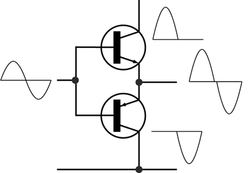
\includegraphics[scale=1]{250px-Electronic_Amplifier_Push-pull.png} 
\end{figure}
\subsection{Funcionamiento de un amplificador de clase B}
Un amplificador de potencia funciona en clase B cuando la polarización de dc deja al transistor casi apagado de manera que el transistor se enciende cuando a este se le aplica una señal en ac. Es decir que le transistor conducirá corriente solamente para una mitad de ciclo de la señal.

Ahora para obtener una señal de ciclo completo será necesario utilizar dos transistores y lograr que cada uno de ellos conduzca durante medios ciclos opuestos, y al tener esta operación combinada se obtiene un ciclo completo de señal de salida.

Dado que una parte del circuito "empuja" a la señal de arriba durante una mitad del ciclo y la otra parte "jala" la señal hacia abajo durante la otra mitad del ciclo, el circuito por ende se denomina de contrafase circuito push-pull.
Los transistores de potencia empleados en el circuito de contrafase son capaces de entregar la potencia deseada a la carga, y la operación clase B de estos transistores proporciona una diferencia mayor que la que era posible mediante un solo transistor en la operación clase A.
\newpage
En un amplificador de potencia con etapa de salida tipo B, debe estar compuesta por dos
etapas complementarias. Cada una de ellas se encuentra sin conducir cuando no hay señal,
y cuando la señal varía respecto de cero hace que conduzca una de las etapas de acuerdo
con la polaridad de la variación. 
\begin{figure}[h!]
\centering
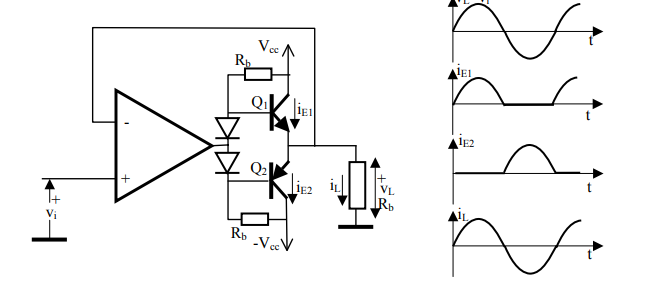
\includegraphics[scale=1]{Captura.PNG} 
\end{figure}
En un amplificador de potencia con etapa de salida tipo B, debe estar compuesta por dos
etapas complementarias. Cada una de ellas se encuentra sin conducir cuando no hay señal,
y cuando la señal varía respecto de cero hace que conduzca una de las etapas de acuerdo
con la polaridad de la variación.
\section{Bibliografias:}
[1] Boylestad Nashelsky, Electronica teoría de circuitos y dispositivos electrónicos, editorial Perason, 8va edición , Pag 761-769

[2] Albert Malvino, Principios de electrónica, editorial Mc Graw Hill ,6ta edición , Pag 395 
\begin{figure}[h!]
\centering
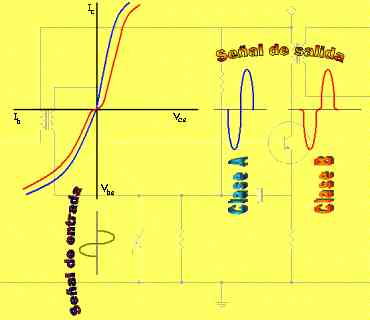
\includegraphics[scale=.5]{generalidades.jpg} 
\end{figure}
\end{document}
